\chapter{Implementierung}
\label{chap:implementierung}

\section{Technologische Basis}
Die Implementierung basiert auf einer sorgfältig ausgewählten technologischen Basis, die modernste Tools und Frameworks kombiniert, um eine effiziente und skalierbare Lösung zu gewährleisten. Die wichtigsten Technologien sind:
\begin{itemize}
    \item \textbf{Frontend:} Entwicklung mit React und TypeScript. Material-UI wird für konsistente UI-Komponenten genutzt, während Vite für schnelle Build- und Entwicklungsprozesse sorgt.
    \item \textbf{Backend:} Aufbau von RESTful APIs mit .NET Core. Middleware-Services ermöglichen Authentifizierung, Fehlerbehandlung und Protokollierung.
    \item \textbf{Datenbank:} Relationale Modellierung und Abfragen in Azure SQL mit Entity Framework Core für nahtlosen Datenzugriff.
    \item \textbf{DevOps:} Automatisierte CI/CD-Pipelines mit Azure Pipelines, die den Entwicklungs- und Bereitstellungsprozess optimieren.
\end{itemize}

\section{Detailierte Architektur}
\subsection{Frontend-Architektur}
Das Frontend wurde mit einer komponentenbasierten Architektur entwickelt, die eine modulare und wiederverwendbare Struktur ermöglicht:
\begin{itemize}
    \item \textbf{Komponenten:} Jedes UI-Element wurde als eigenständige Komponente entwickelt, um Wartbarkeit und Wiederverwendbarkeit zu maximieren.
    \item \textbf{State-Management:} Für die Verwaltung globaler Zustände kommen Redux Toolkit und Zustand zum Einsatz.
    \item \textbf{Datenvisualisierung:} ApexCharts und React-ApexCharts werden zur Darstellung von Donut- und Radarcharts verwendet.
\end{itemize}

\begin{minted}[linenos, frame=single, fontsize=\small, caption=Beispiel einer React-Komponente, label=lst:react_component]{javascript}
import React from 'react';
import { Chart } from 'react-apexcharts';

const RadarChart = () => {
  const data = {
    labels: ['Teamarbeit', 'Effizienz', 'Pünktlichkeit', 'Innovation'],
    datasets: [
      {
        label: 'Mitarbeiter A',
        data: [80, 90, 70, 85],
        backgroundColor: 'rgba(54, 162, 235, 0.2)',
        borderColor: 'rgba(54, 162, 235, 1)',
        borderWidth: 2,
      },
    ],
  };

  return <Chart options={data} type="radar" />;
};

export default RadarChart;
\end{minted}


\section{Backend-Architektur}
Das Backend basiert auf einer mehrschichtigen Architektur, die eine klare Trennung von Verantwortlichkeiten gewährleistet. Diese Architektur stellt die Grundlage für eine effiziente und skalierbare Verarbeitung von Mitarbeitendengesprächsdaten dar.

\subsection{Technologische Basis}
Die Entwicklung des Backends erfordert eine fundierte Auswahl moderner Technologien und Methoden, um zentrale Anforderungen wie Sicherheit, Performanz, Skalierbarkeit und Datenverarbeitung zu erfüllen. Folgende Komponenten sind integraler Bestandteil der Implementierung:
\begin{itemize}
    \item \textbf{API-Entwicklung:} Implementierung von RESTful APIs mit .NET Core, die eine zuverlässige und standardisierte Datenübertragung ermöglichen.
    \item \textbf{Cloud-Technologien:} Integration von Microsoft Azure-Diensten wie Azure SQL und Azure Service Bus zur Unterstützung asynchroner Kommunikation und Datenverarbeitung.
    \item \textbf{Sicherheitsmechanismen:} Einsatz von Azure Active Directory (AAD) für Multi-Faktor-Authentifizierung und rollenbasierte Zugriffskontrolle.
    \item \textbf{Datenverarbeitung:} Nutzung skalierbarer Algorithmen zur Aggregation und Transformation komplexer Datenstrukturen.
\end{itemize}

\subsection{Komponenten der Backend-Architektur}
\begin{itemize}
    \item \textbf{Controller-Schicht:} Zuständig für die Verarbeitung von Anfragen und das Routing.
    \item \textbf{Service-Schicht:} Implementiert die Geschäftslogik und ist für Datenverarbeitung und Validierung verantwortlich.
    \item \textbf{Repository-Schicht:} Ermöglicht den Zugriff auf die Datenbank mithilfe von Entity Framework Core.
    \item \textbf{Middleware:} Authentifizierung und Fehlerbehandlung werden zentral über Middleware-Komponenten gesteuert.
\end{itemize}

\begin{lstlisting}[language=C, caption=Beispiel eines .NET Core Controllers, label=lst:dotnet_controller]
[ApiController]
[Route("api/[controller]")]
public class EmployeeController : ControllerBase
{
    private readonly EmployeeService _employeeService;

    public EmployeeController(EmployeeService employeeService)
    {
        _employeeService = employeeService;
    }

    [HttpGet("{id}")]
    public async Task<IActionResult> GetEmployeeById(int id)
    {
        var employee = await _employeeService.GetEmployeeByIdAsync(id);
        if (employee == null)
        {
            return NotFound();
        }
        return Ok(employee);
    }
}
\end{lstlisting}

\subsection{Sicherheitsmechanismen und Skalierbarkeit}
Die Sicherheitsmechanismen des Backends gewährleisten die Integrität und Vertraulichkeit sensibler Daten. Hierzu zählen:
\begin{itemize}
    \item \textbf{Authentifizierung:} Azure Active Directory ermöglicht Multi-Faktor-Authentifizierung und Single Sign-On.
    \item \textbf{Datenverschlüsselung:} Sensible Daten werden durch AES-256 sowohl im Ruhezustand als auch während der Übertragung geschützt.
    \item \textbf{Rollenbasierte Zugriffskontrolle:} Strikte Zugriffsrichtlinien stellen sicher, dass nur autorisierte Personen auf spezifische Daten zugreifen können.
\end{itemize}

\subsection{Integration von Microsoft Azure-Diensten}
Die Einbindung von Microsoft Azure-Diensten spielt eine zentrale Rolle in der Backend-Entwicklung:
\begin{itemize}
    \item \textbf{Azure SQL:} Bereitstellung einer skalierbaren und sicheren Plattform für die Speicherung großer Mengen sensibler Daten.
    \item \textbf{Azure Service Bus:} Unterstützung asynchroner Kommunikationsprozesse zwischen Systemkomponenten.
    \item \textbf{Automatisierung:} Erstellung automatisierter Berichte und datenbasierter Einblicke aus den gespeicherten Gesprächsdaten.
\end{itemize}

\subsection{Optimierung der Datenverarbeitung}
Durch die Implementierung moderner Algorithmen wird die Verarbeitung komplexer Datenstrukturen optimiert:
\begin{itemize}
    \item \textbf{Natural Language Processing (NLP):} Analyse unstrukturierter Gesprächsnotizen zur Erkennung von Mustern und Trends.
    \item \textbf{Datenaggregation:} Konsolidierung unterschiedlicher Quellen zur Erstellung ganzheitlicher Analysen.
\end{itemize}

\subsection{Überwachung und Wartbarkeit}
Eine modulare Architektur unterstützt die Wartbarkeit und Überwachung des Systems:
\begin{itemize}
    \item \textbf{Monitoring:} Ein spezifisches Monitoring-System identifiziert Leistungseinbußen und sendet Warnmeldungen.
    \item \textbf{Automatisierte Tests:} Sicherstellung der Funktionsfähigkeit durch kontinuierliche Integration und Tests.
    \item \textbf{Containerisierung:} Verwendung von Docker, um Konsistenz zwischen Entwicklungs- und Produktionsumgebungen sicherzustellen.
\end{itemize}

\subsection{Zusammenfassung}
Die Backend-Entwicklung kombiniert moderne Technologien und Sicherheitsmechanismen, um eine leistungsfähige, skalierbare und sichere Plattform zur Visualisierung von Mitarbeitendengesprächsdaten bereitzustellen. Durch die Integration von Cloud-Diensten, robusten Algorithmen und einer modularen Architektur wird eine optimale Nutzererfahrung gewährleistet.


\subsection{Datenbankmodell}
Die relationale Datenbank wurde mit Azure SQL implementiert. Wichtige Tabellen und deren Beziehungen sind in Abbildung~\ref{fig:db_er_model} dargestellt. Das Schema wurde so gestaltet, dass es sowohl aktuelle als auch historische Daten effizient speichern kann.

\begin{figure}[h!]
    \centering
    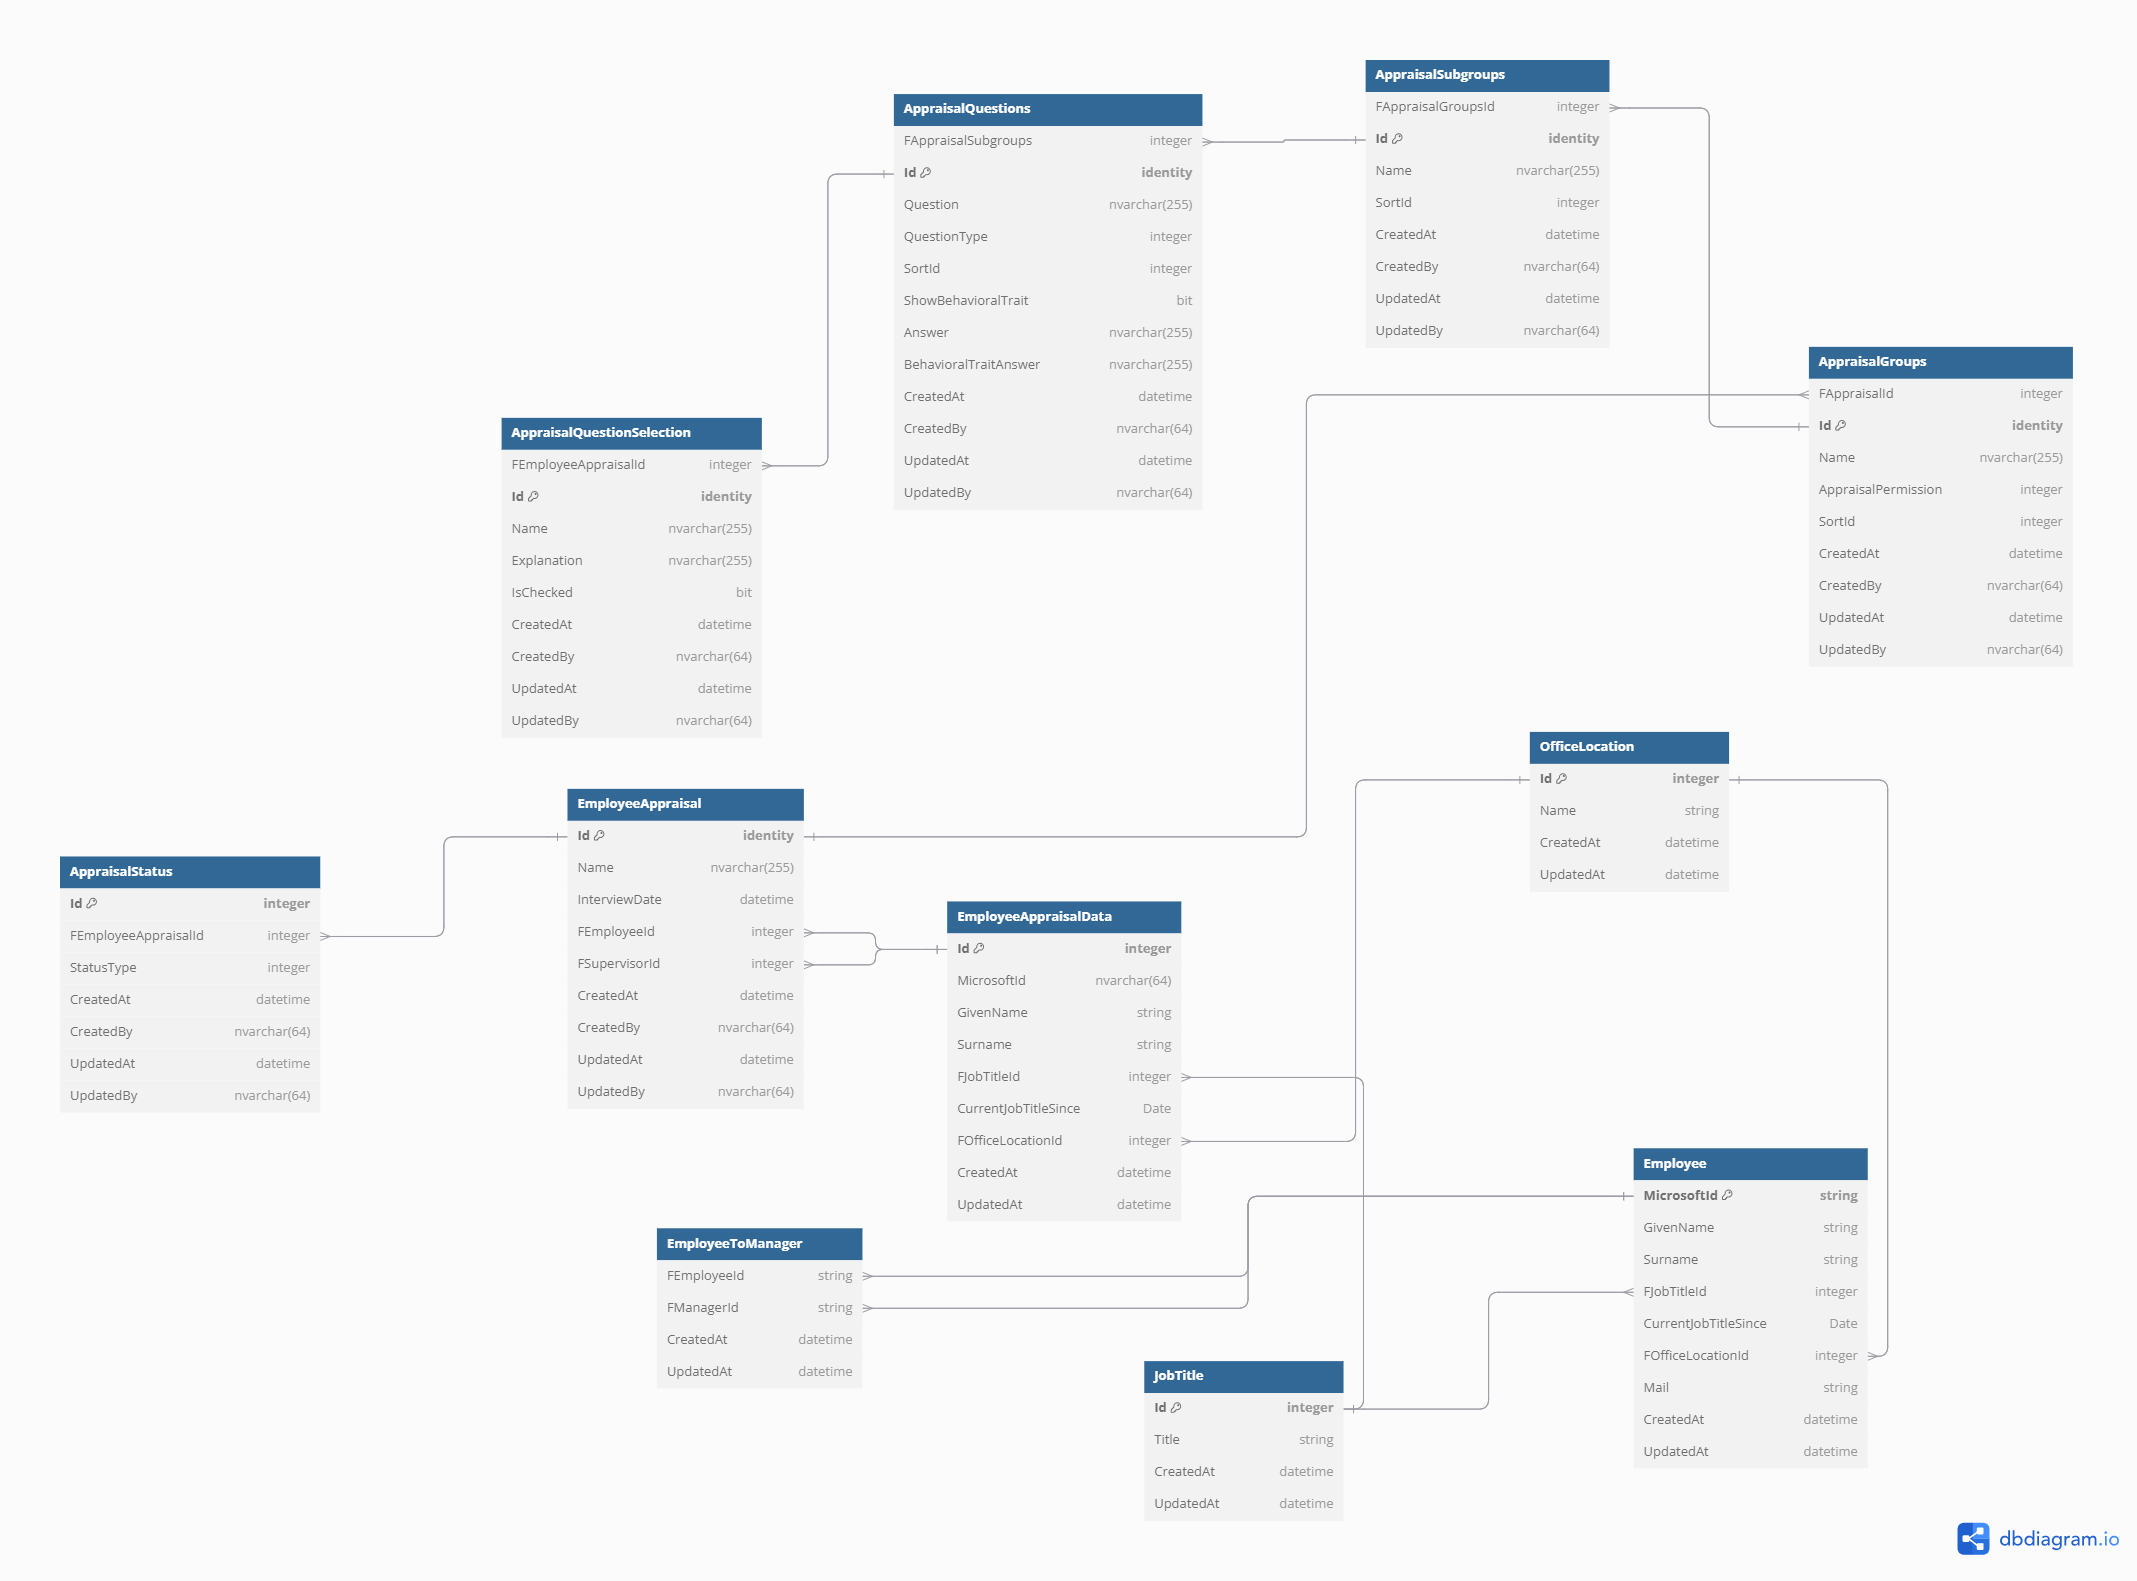
\includegraphics[width=0.8\textwidth]{images/er_modell_design.png}
    \caption{ER-Diagramm der Datenbankstruktur.}
    \label{fig:db_er_model}
\end{figure}

\section{Herausforderungen und Lösungen}
\subsection{Datenkonsistenz}
Um die Konsistenz der Daten zu gewährleisten, wurde eine Transaktionsverwaltung implementiert. Dies verhindert Dateninkonsistenzen bei parallelen Datenbankoperationen.

\subsection{Echtzeit-Updates}
Mit Azure Service Bus wurde eine asynchrone Kommunikation ermöglicht. Dies erlaubt Echtzeit-Benachrichtigungen an Benutzer, ohne die Backend-Leistung zu beeinträchtigen.

\subsection{Optimierung der Benutzerfreundlichkeit}
Durch regelmäßige Usability-Tests und die iterative Anpassung der UI-Elemente wurde die Benutzerfreundlichkeit kontinuierlich verbessert.

\section{Test- und Debugging-Prozesse}
\subsection{Frontend-Tests}
Komponenten wurden mit Jest und React Testing Library getestet, um deren Funktionalität und Robustheit sicherzustellen.

\subsection{Backend-Tests}
Die RESTful APIs wurden mit Postman und automatisierten Integrationstests getestet.

\subsection{Debugging}
Entwicklerwerkzeuge wie Visual Studio Debugger und Browser DevTools wurden für die Analyse und Behebung von Fehlern verwendet.

\section{Zusammenfassung}
Die Implementierung des Systems kombiniert moderne Technologien, robuste Sicherheitsmaßnahmen und optimierte Workflows. Es bietet eine performante, skalierbare und benutzerfreundliche Lösung, die den Anforderungen moderner HR-Tools gerecht wird.
